\input{permve-ntnu-latex-assignment.tex}

\usepackage{float}

\title{
\normalfont \normalsize
\textsc{Norwegian University of Science and Technology\\TDT4136 -- Introduction to Artificial Intelligence} \\ [25pt]
\horrule{0.5pt} \\[0.4cm]
\huge Assignment 3:\\ Using the A* Algorithm\\
\horrule{2pt} \\[0.5cm]
}

\author{Per Magnus Veierland\\permve@stud.ntnu.no}

\date{\normalsize\today}

\newacro{BFS}{Breadth First Search}

\newcommand{\showboard}[4]{
    \begin{figure}[H]
    \centering
    \includegraphics[width=#4\textwidth]{images/#1-#2}
    \caption{#3}
    \end{figure}
}

\newcommand{\showbfs}[2]{\showboard{#1}{breadth_first}{Breadth First Search}{#2}}
\newcommand{\showdijkstra}[2]{\showboard{#1}{dijkstra}{Dijkstra's Algorithm}{#2}}
\newcommand{\showastar}[2]{\showboard{#1}{astar}{A* Search}{#2}}
\newcommand{\showboards}[2]{\showbfs{#1}{#2}\showdijkstra{#1}{#2}\showastar{#1}{#2}}

\hyphenation{Dijkstra}

\begin{document}

\maketitle

\section*{Problem A: Pathfinding in 2D Games}

The \texttt{a1.py} program visualizes A* search in boards with uniform costs and obstacles for A.1.2. The \texttt{a2.py} program visualizes A* search for boards with different costs for A.2.2. The programs \texttt{a3-a.py} and \texttt{a3-b.py} visualizes search using \texttt{BFS}, Dijkstra's algorithm, and A* search for boards with uniform and non-uniform costs respectively for A.3.2. All programs uses the \texttt{vi} Python library which was developed for the IT3105 module.

\begin{figure}[H]
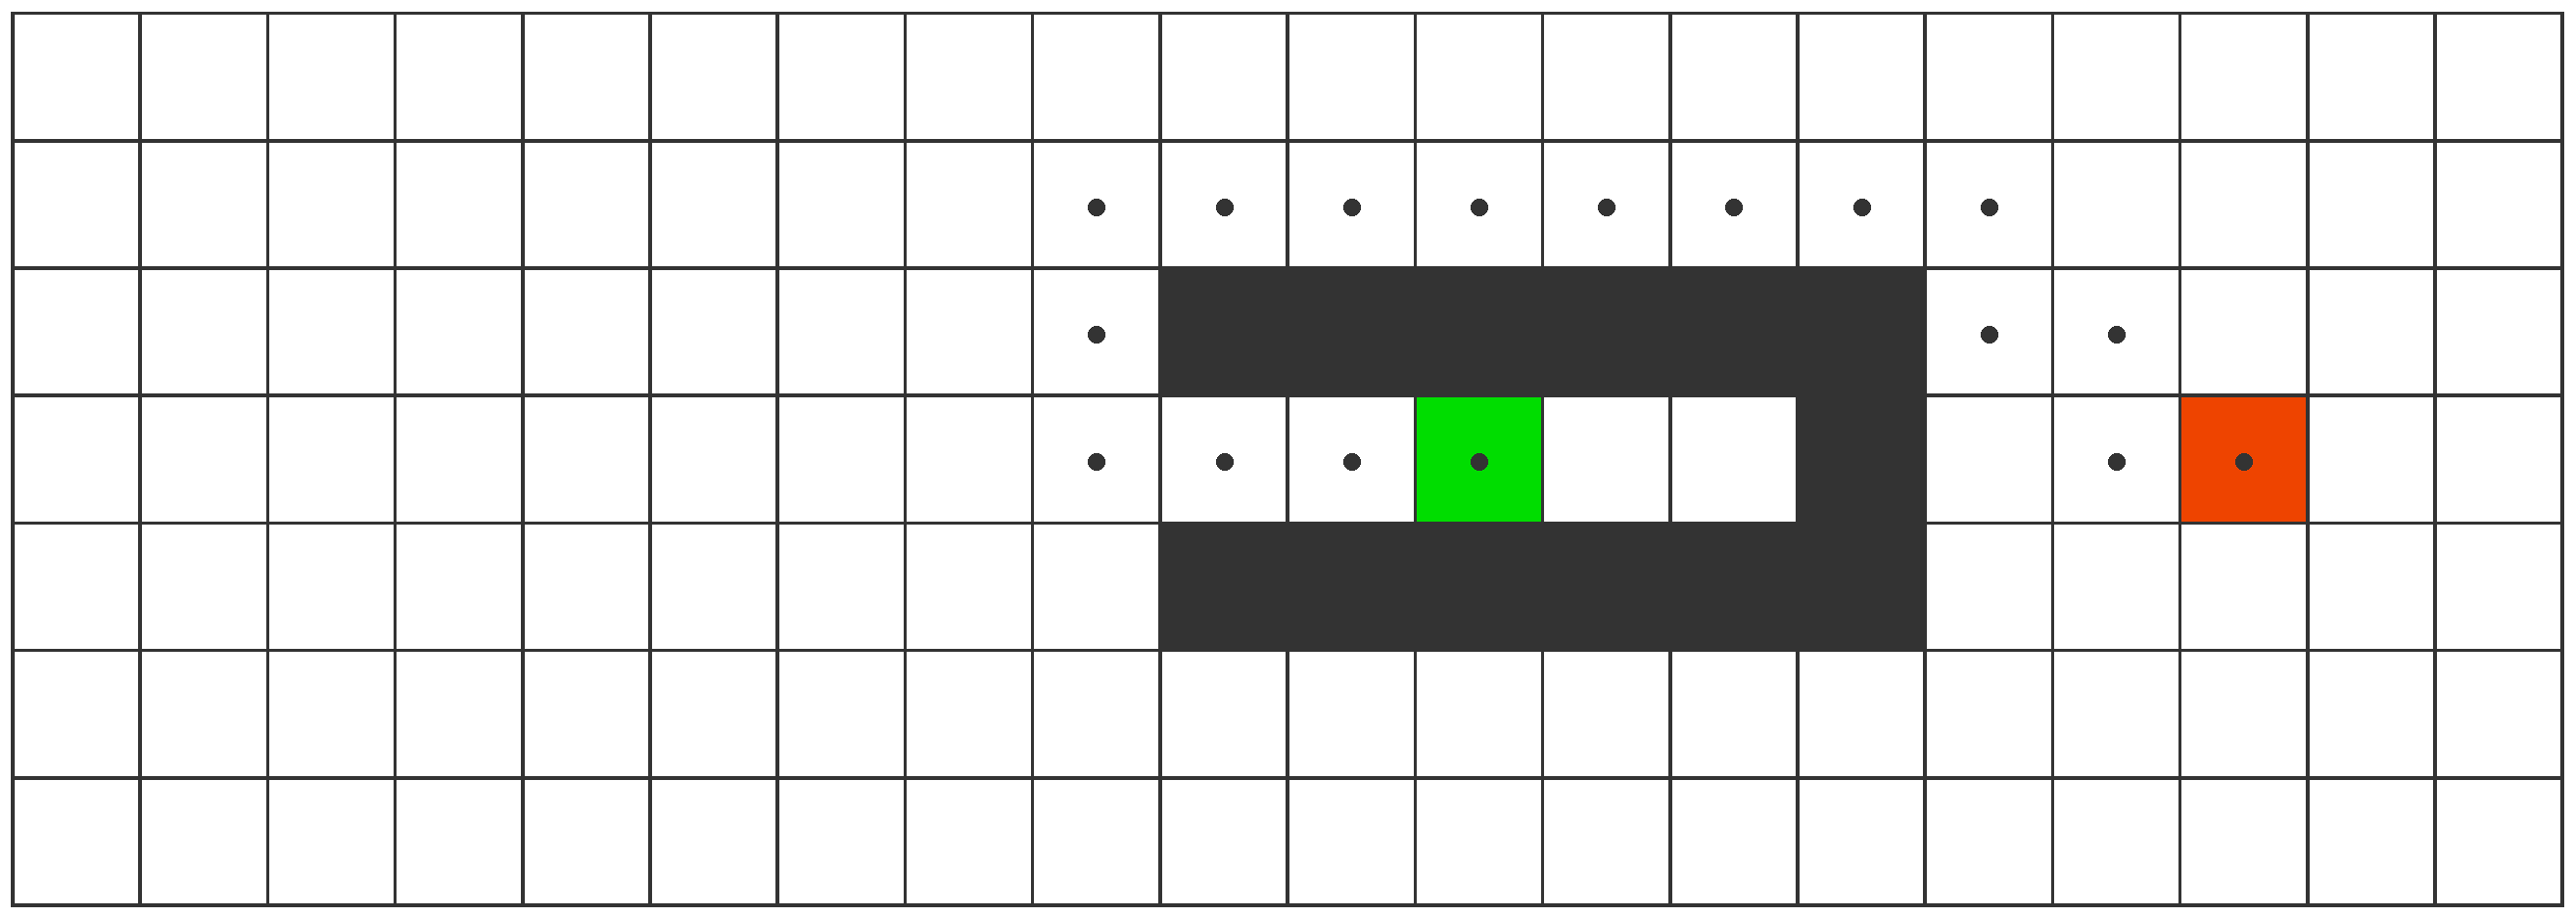
\includegraphics[width=\textwidth]{images/board-1-1}
\caption{\texttt{~board-1-1.txt~}}
\end{figure}

\begin{figure}[H]
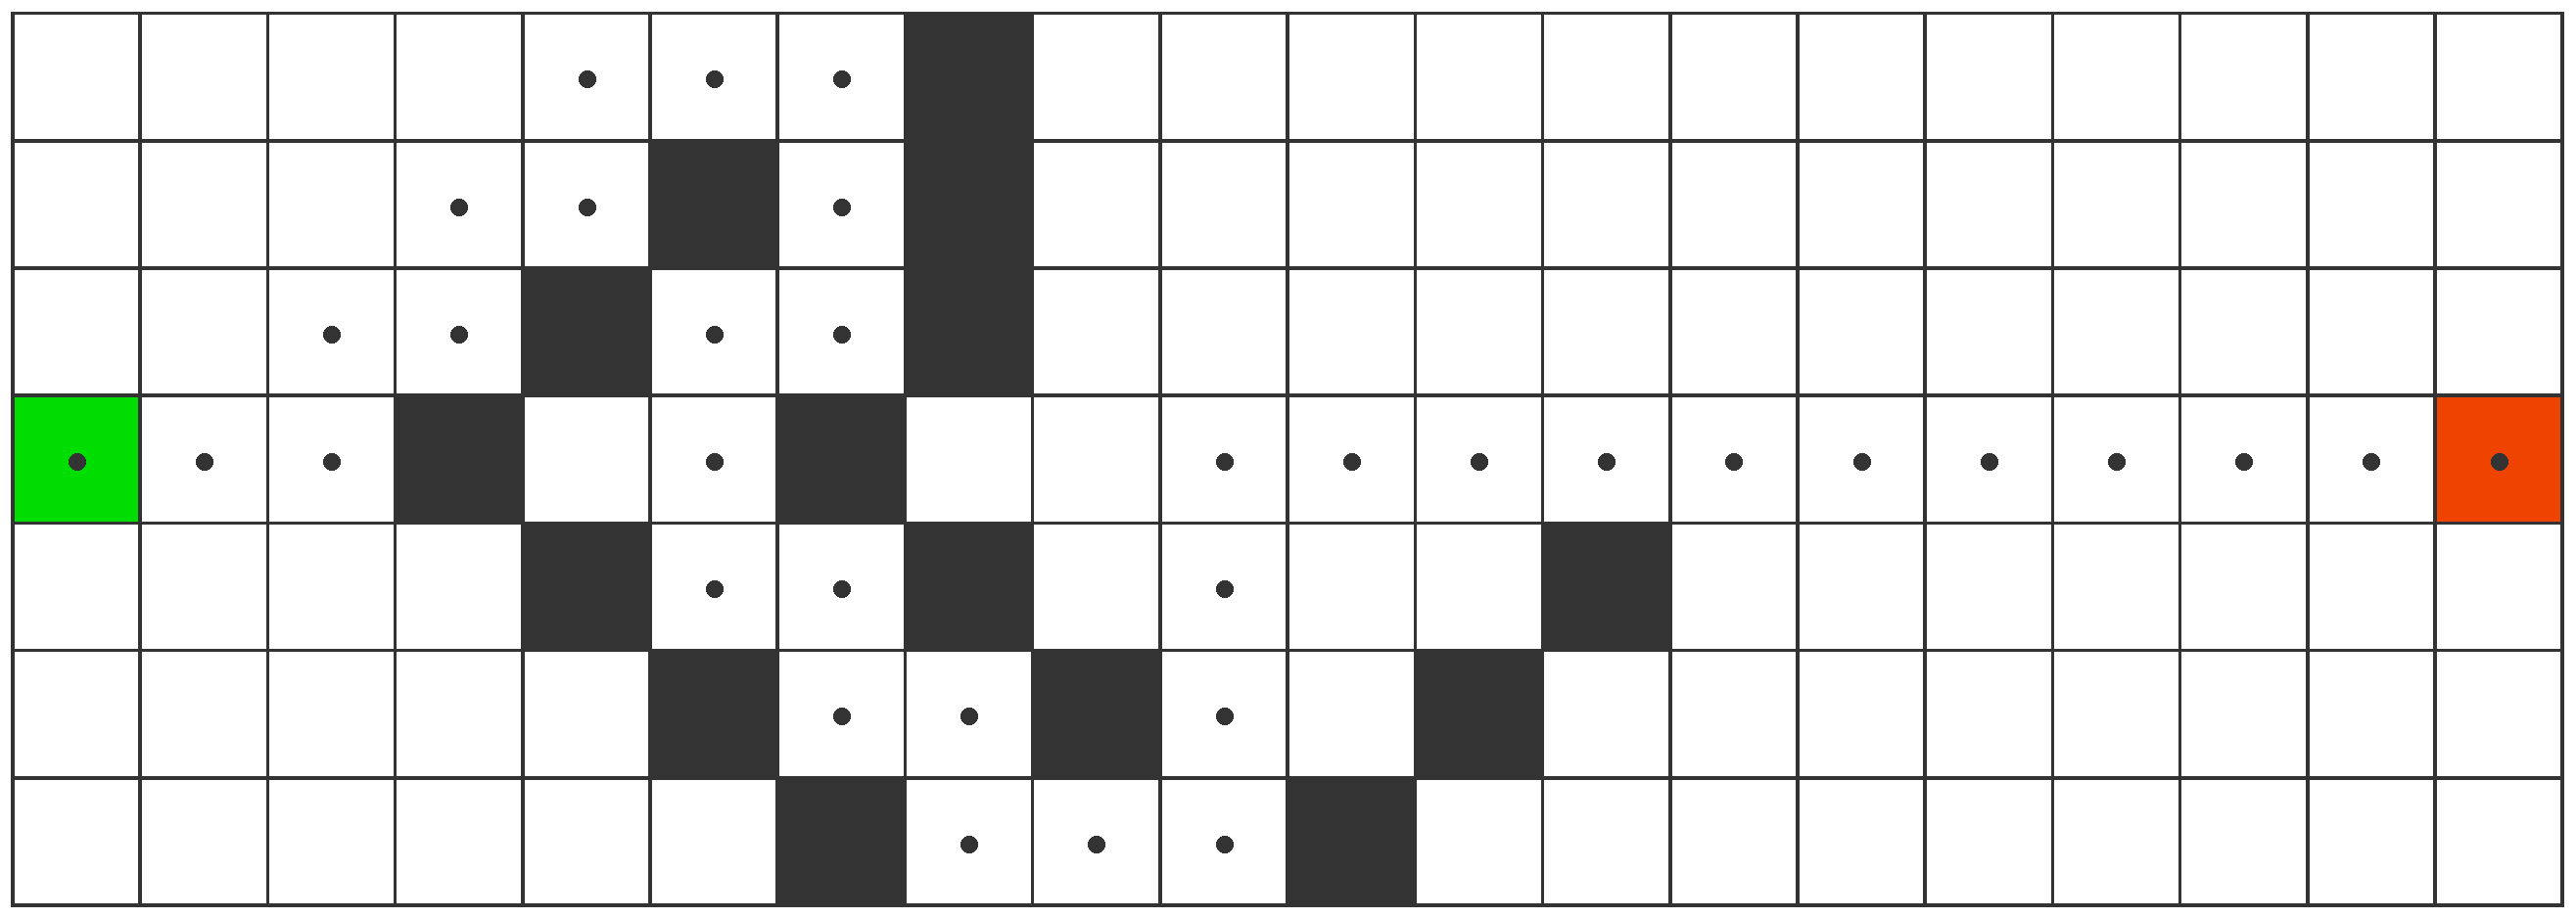
\includegraphics[width=\textwidth]{images/board-1-2}
\caption{\texttt{~board-1-2.txt~}}
\end{figure}

\begin{figure}[H]
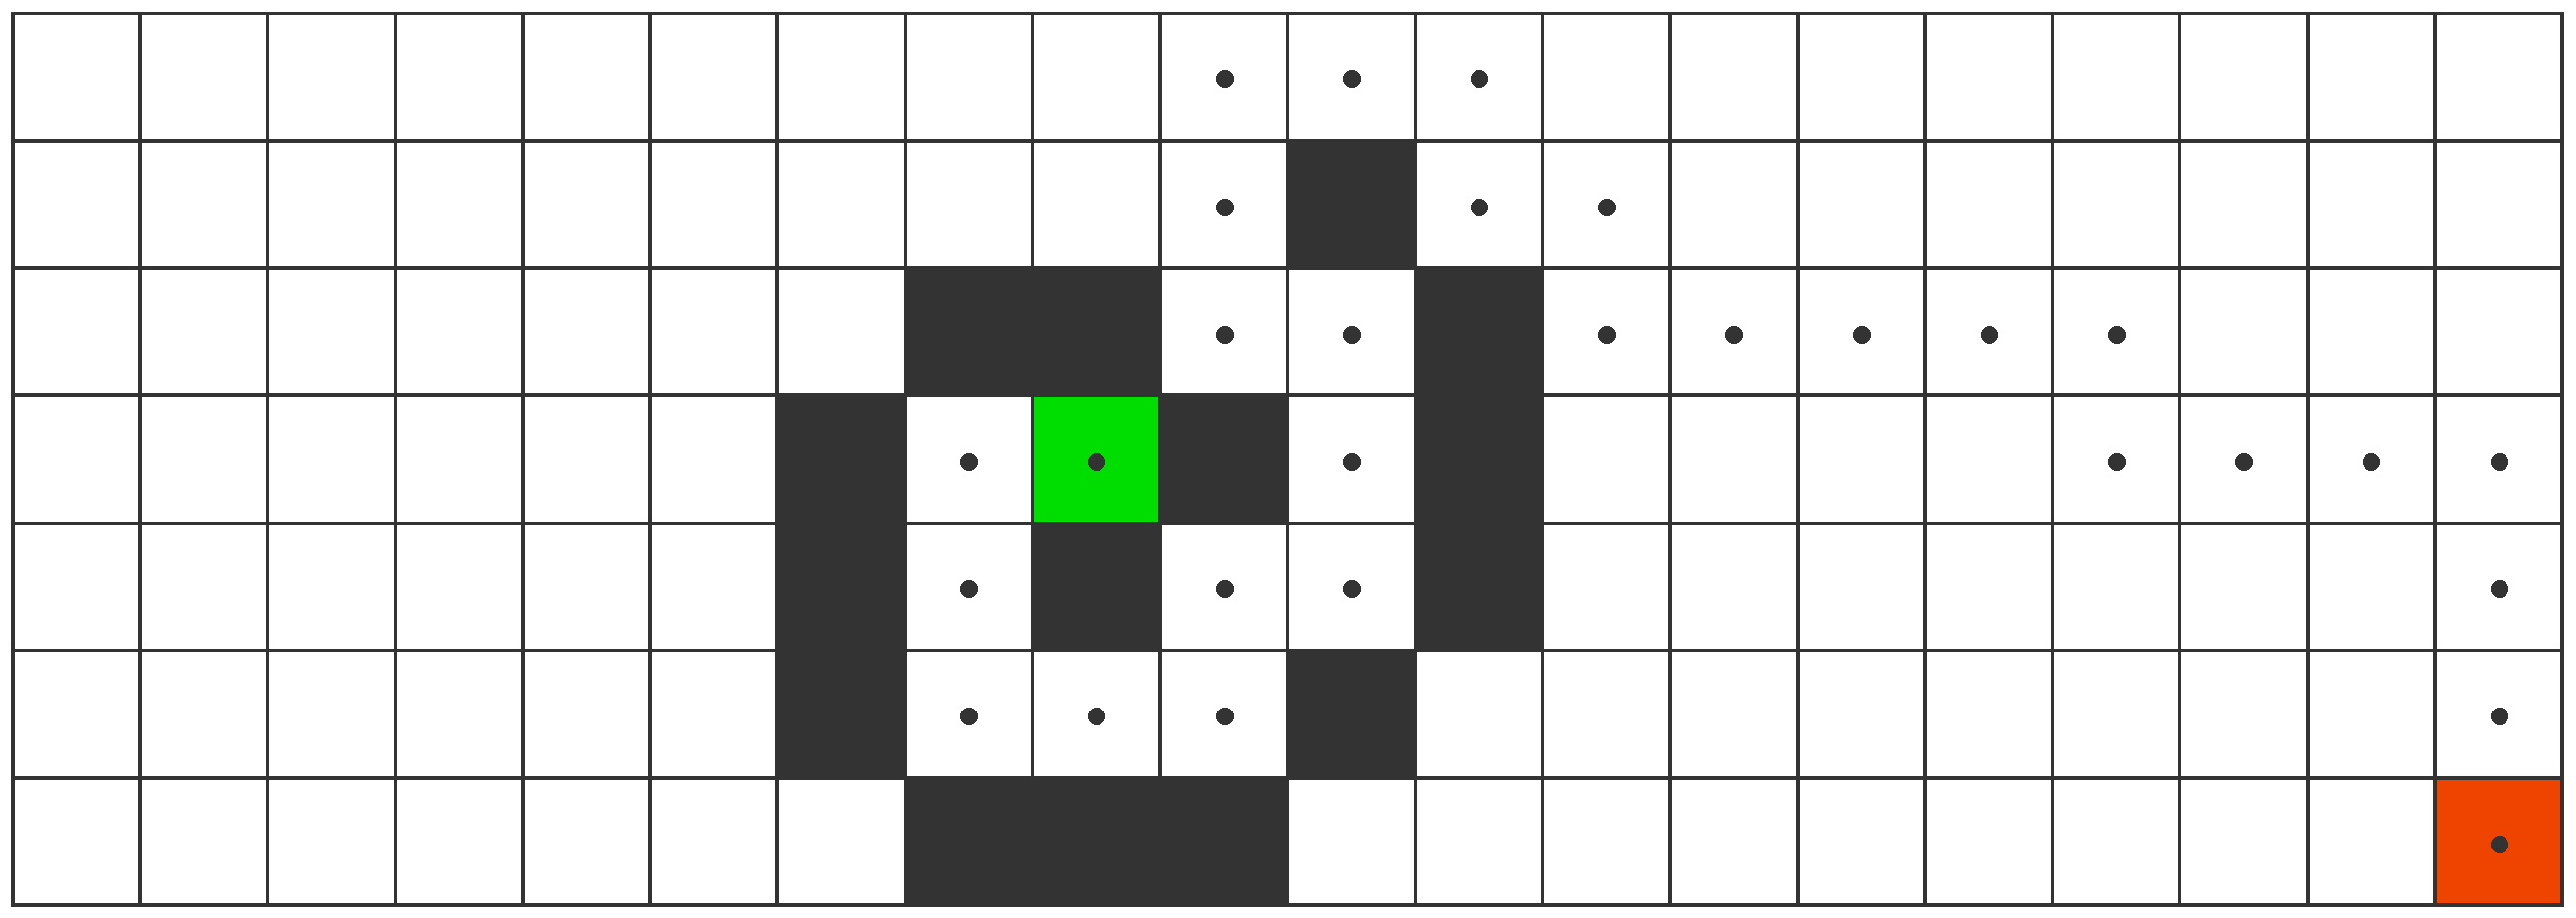
\includegraphics[width=\textwidth]{images/board-1-3}
\caption{\texttt{~board-1-3.txt~}}
\end{figure}

\begin{figure}[H]
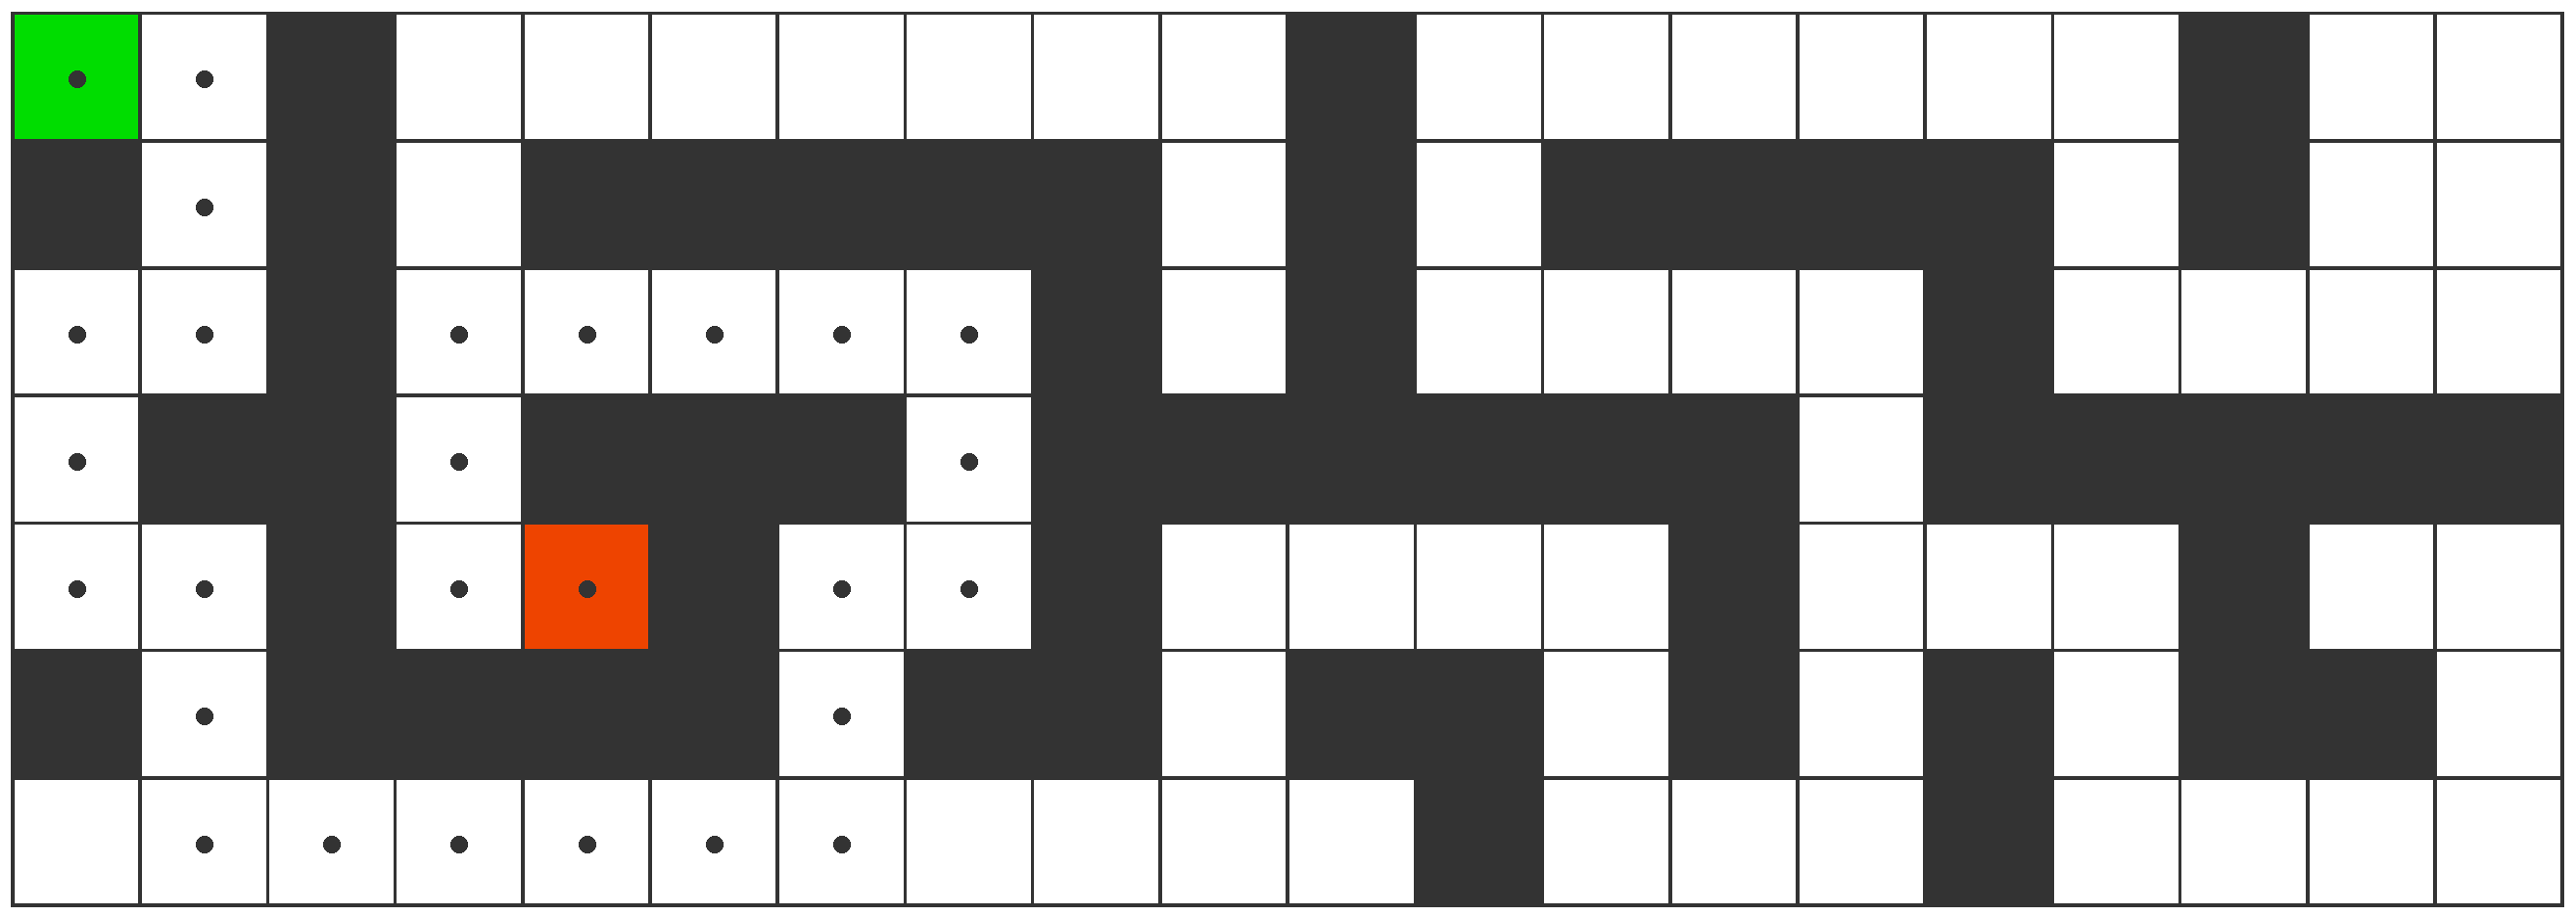
\includegraphics[width=\textwidth]{images/board-1-4}
\caption{\texttt{~board-1-4.txt~}}
\end{figure}

\newpage

\begin{figure}[H]
\centering
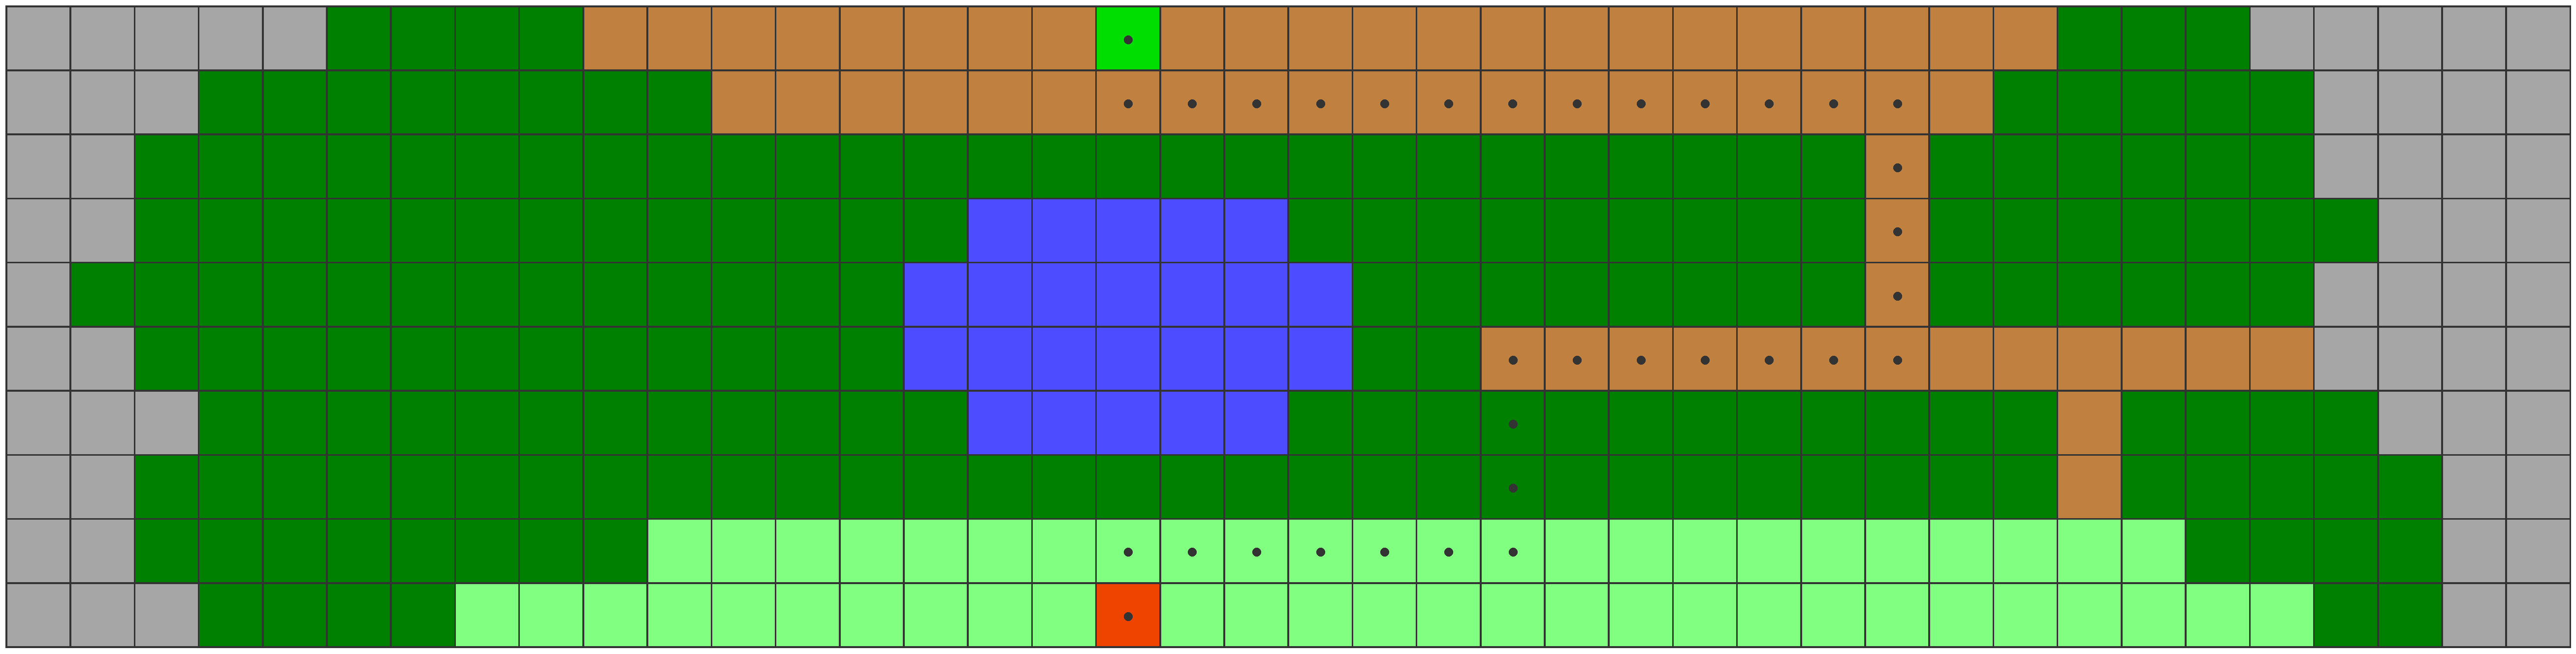
\includegraphics[width=0.9\textwidth]{images/board-2-1}
\caption{\texttt{~board-2-1.txt~}}
\end{figure}

\begin{figure}[H]
\centering
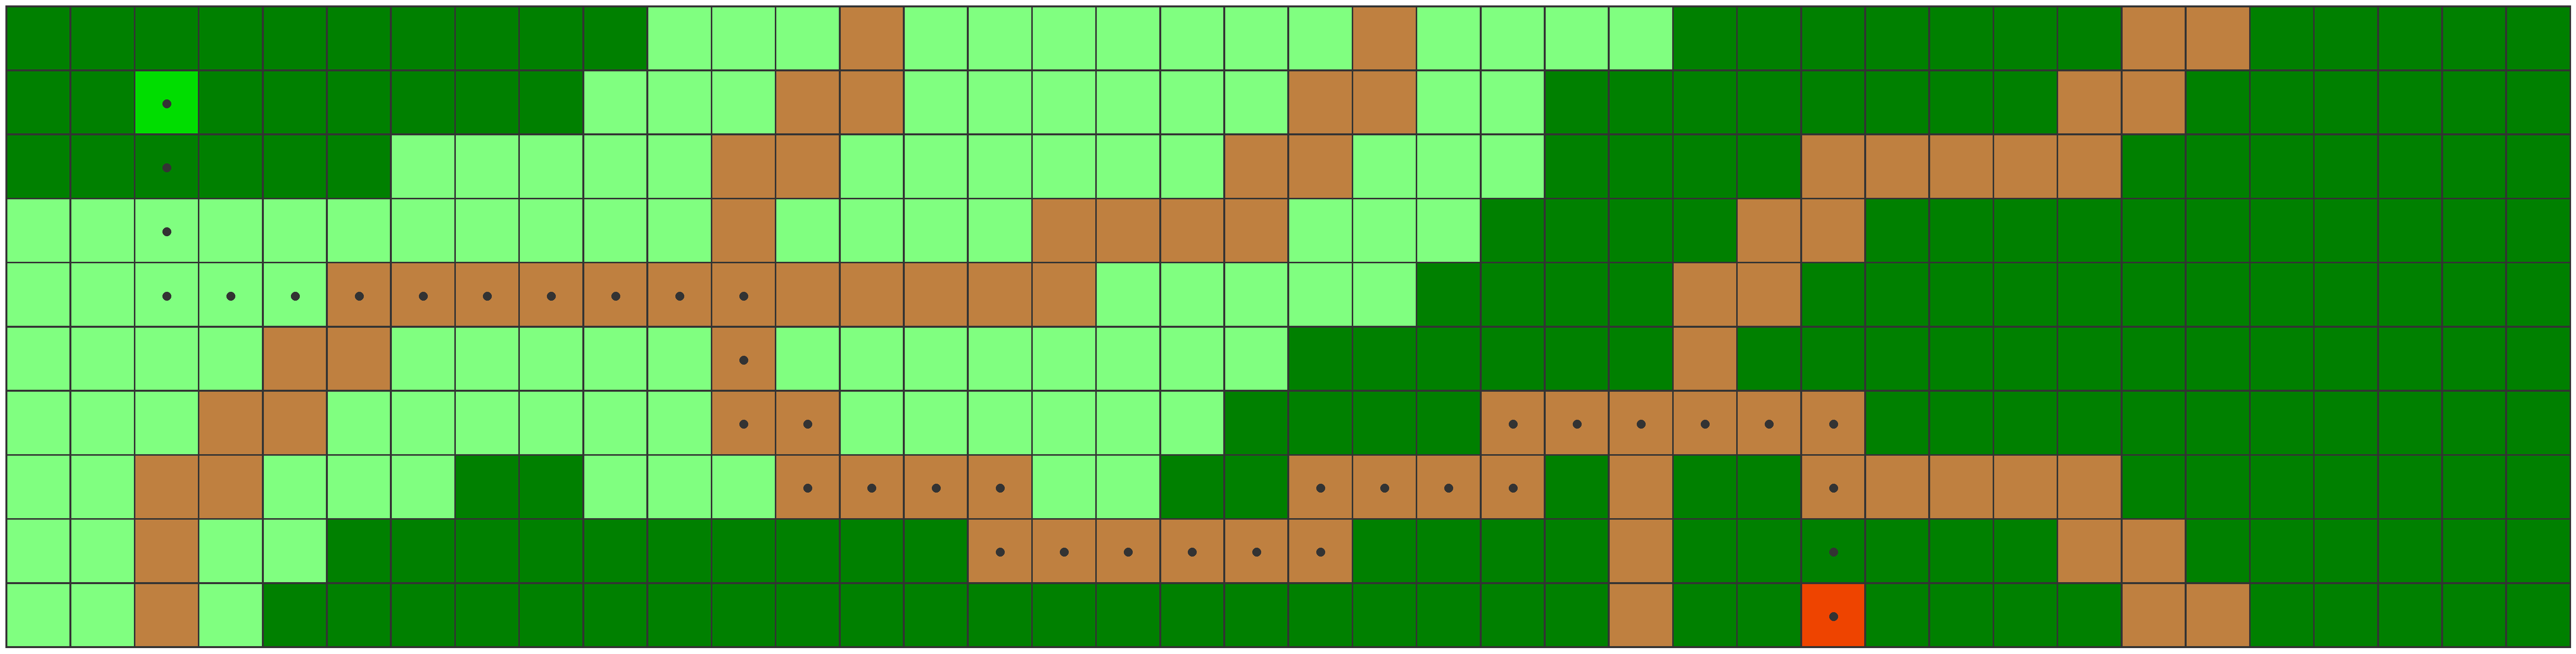
\includegraphics[width=0.9\textwidth]{images/board-2-2}
\caption{\texttt{~board-2-2.txt~}}
\end{figure}

\begin{figure}[H]
\centering
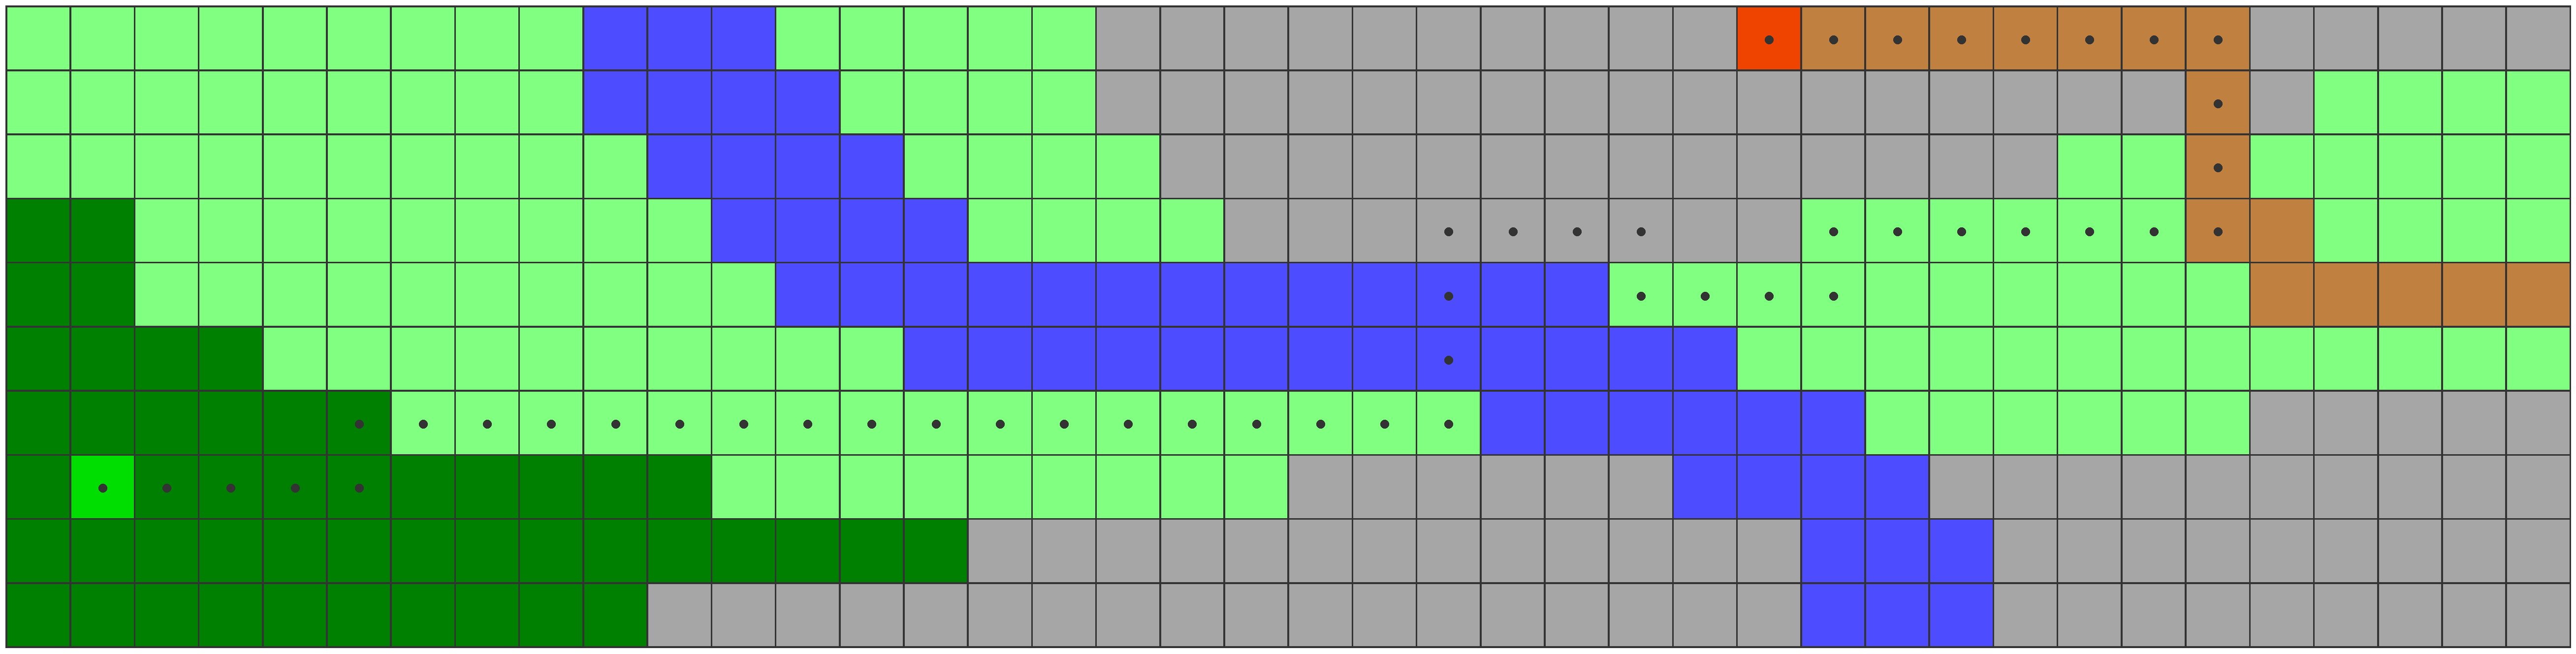
\includegraphics[width=0.9\textwidth]{images/board-2-3}
\caption{\texttt{~board-2-3.txt~}}
\end{figure}

\begin{figure}[H]
\centering
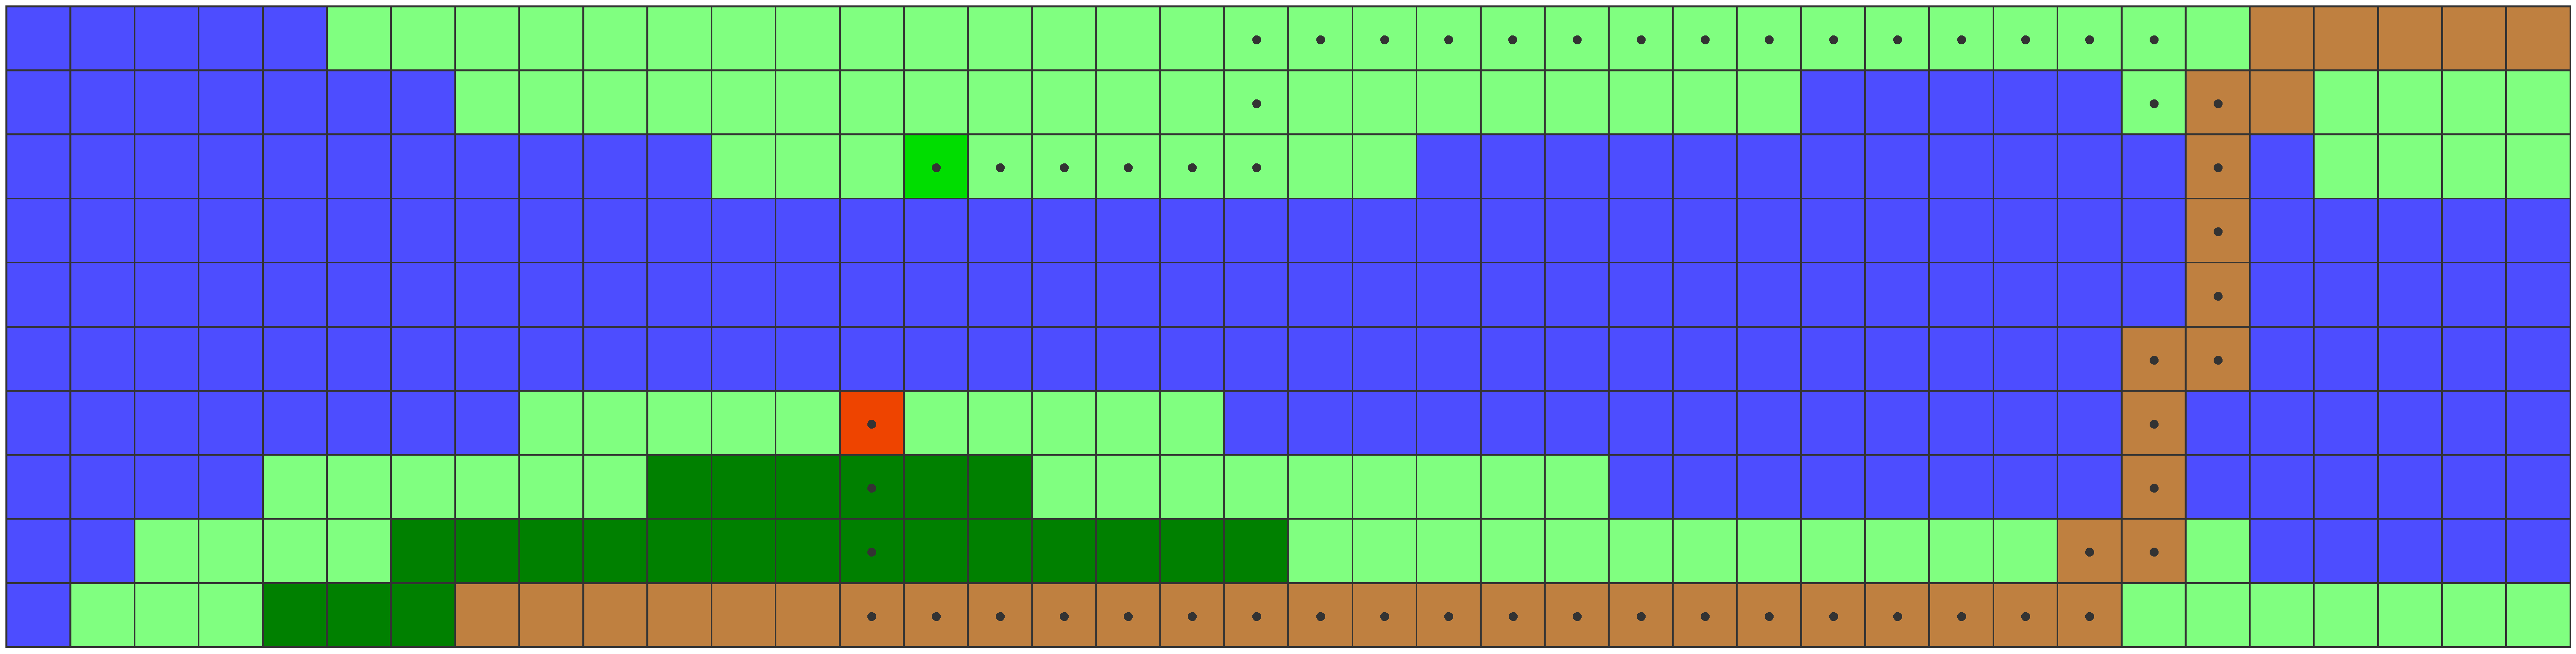
\includegraphics[width=0.9\textwidth]{images/board-2-4}
\caption{\texttt{~board-2-4.txt~}}
\end{figure}

\newpage
\subsection*{A.3.3 -- Board-1-1}

Both \ac{BFS} and Dijkstra consider a large number of states and perform almost identically. The A* strategy considers significantly fewer states, but evaluates both symmetrical possible paths to the goal. All three strategies produce optimal paths.

\showboards{board-1-1}{0.75}

\newpage
\subsection*{A.3.3 -- Board-1-2}

Both \ac{BFS} and Dijkstra consider a large number of states and perform almost identically. The A* strategy considers all nodes before the obstacle; but after exiting the obstacle it moves in a straight line towards the goal due to its heuristic. All three strategies produce optimal paths.

\showboards{board-1-2}{0.75}

\newpage
\subsection*{A.3.3 -- Board-1-3}

Both \ac{BFS} and Dijkstra consider all states in the grid. The A* strategy considers significantly fewer nodes and none after the center obstacle. Gaps of states on the ``open list'' in the right grid area can be seen for A* due to its Manhattan heuristic. All three strategies produce optimal paths.

\showboards{board-1-3}{0.75}

\newpage
\subsection*{A.3.3 -- Board-1-4}

It can be seen than \ac{BFS} and Dijkstra consider the same number of nodes; and that they continue the searches in non-goal directions further than A*. All three strategies produce optimal paths.

\showboards{board-1-4}{0.75}

\newpage
\subsection*{A.3.3 -- Board-2-1}

When boards with non-uniform costs are introduced; the difference between \ac{BFS} and Dijkstra's algorithm becomes clear. \ac{BFS} follows all states outwards from the start and ignores costs. It finds the straight path to the goal; however this path is sub-optimal since costs are not uniform. Both Dijkstra and A* finds optimal paths; however A* considers slightly fewer states.

\showboards{board-2-1}{1}

\newpage
\subsection*{A.3.3 -- Board-2-2}

The \ac{BFS} search chooses a straight path which ignores path costs and ends up being quite suboptimal. Both Dijkstra's algorithm and A* search finds the optimal paths; but Dijkstra's algorithm considers a few more states than A* due to its lack of a heuristic.

\showboards{board-2-2}{1}

\newpage
\subsection*{A.3.3 -- Board-2-3}

The \ac{BFS} appears to do well in this scenario and finds a path close to the optimal. However it still traverses more water cells and mountain cells than the optimal path. Both Dijkstra's algorithm and A* search finds the optimal paths; but Dijkstra's algorithm considers a few more states than A* due to its lack of a heuristic.

\showboards{board-2-3}{1}

\newpage
\subsection*{A.3.3 -- Board-2-4}

The \ac{BFS} search traverses states equally in all directions and finds the path to the goal which is the fewest number of states away; but which has a much greater path cost than the optimal path. Both Dijkstra's algorithm and A* search finds the optimal paths; but Dijkstra's algorithm considers a few more states than A* due to its lack of a heuristic.

\showboards{board-2-4}{1}

\newpage
\section*{Problem B: Rush Hour Puzzle}

\begin{enumerate}[label=B.\arabic*:]
\item The program \texttt{rush\_hour.py} contains a solution for the Rush Hour puzzle using A* search by utilizing the \texttt{vi} Python library developed for IT3105.
\item Two heuristics were developed for the Rush Hour puzzle:

\textit{Heuristic \#1} is calculated as the distance between \textit{Car \#0} and the goal coordinate. This heuristic is guaranteed to be admissible, since \textit{Car \#0} must be moved to the goal in order for the puzzle to be solved. Even if this is a very basic heuristic, it is easy to implement and cheap to evaluate. Table~\ref{table:rush_hour_heuristics} shows that it reduces the number of nodes generated by 3\%, 14\%, 27\%, and 20\% respectively in the 4 scenarios given.

\textit{Heuristic \#2} is calculated as the distance between \textit{Car \#0} and the goal coordinate, plus 1 for each of the occupied cells between \textit{Car \#0} and the goal. This heuristic is also guaranteed to be admissible for the same reason as \textit{Heuristic \#1}, and because each occupied cell between \textit{Car \#0} and the goal will at least require 1 move in order to move the blocking car out of the way. This is also a very basic heuristic, but again it is easy to implement and cheap to evaluate. Table~\ref{table:rush_hour_heuristics} shows that it reduces the number of nodes generated by 8\%, 21\%, 49\%, and 41\% respectively in the 4 scenarios given.

\item Successor states are generated from a given state by individually moving all vehicles in the state one step in both directions of their orientation, given that the move is into an unobstructed space. Each successor state only consists of one individual movement of one car.
\end{enumerate}

\begin{table}
\centering
\begin{tabular}{lccccccc}
\toprule
& & \multicolumn{3}{c}{Search Cost (nodes generated)} & \multicolumn{3}{c}{Effective Branching Factor} \\
Scenario & $d$ & Dijkstra & A*$(h_1)$ & A*$(h_2)$ & Dijkstra & A*$(h_1)$ & A*$(h_2)$ \\
\midrule
\textsc{Easy-3}   & 16 &    97 &   94 &   89 & 1.192 & 1.189 & 1.183 \\
\textsc{Medium-1} & 24 &   829 &  710 &  656 & 1.235 & 1.225 & 1.221 \\
\textsc{Hard-3}   & 33 &  2050 & 1504 & 1046 & 1.192 & 1.179 & 1.163 \\
\textsc{Expert-2} & 73 & 11226 & 8925 & 6600 & 1.100 & 1.095 & 1.090 \\
\bottomrule
\end{tabular}
\caption{Rush Hour heuristic comparison}
\label{table:rush_hour_heuristics}
\end{table}

\newpage
\subsection*{B.4 -- Easy-3}
\nobreak
\centering Rush Hour scenario \textsc{Easy-3} can be optimally solved in 16 moves.
\begin{longtable}{rl}
\textbf{Step 1-2:} & Move vehicle \#0 left 2 steps. \\
\textbf{Step 3-4:} & Move vehicle \#4 down 2 steps. \\
\textbf{Step 5-8:} & Move vehicle \#3 left 4 steps. \\
\textbf{Step 9-10:} & Move vehicle \#4 up 2 steps. \\
\textbf{Step 11-12:} & Move vehicle \#0 right 2 steps. \\
\textbf{Step 13-14:} & Move vehicle \#5 up 2 steps. \\
\textbf{Step 15-16:} & Move vehicle \#0 right 2 steps. \\
\end{longtable}

\subsection*{B.4 -- Medium-1}
\nobreak
\centering Rush Hour scenario \textsc{Medium-1} can be optimally solved in 24 moves.
\begin{longtable}{rl}
\textbf{Step 1:} & Move vehicle \#10 down 1 step. \\
\textbf{Step 2:} & Move vehicle \#9 down 1 step. \\
\textbf{Step 3:} & Move vehicle \#3 right 1 step. \\
\textbf{Step 4:} & Move vehicle \#6 up 1 step. \\
\textbf{Step 5:} & Move vehicle \#8 down 1 step. \\
\textbf{Step 6-7:} & Move vehicle \#0 right 2 steps. \\
\textbf{Step 8:} & Move vehicle \#5 down 1 step. \\
\textbf{Step 9-10:} & Move vehicle \#4 up 2 steps. \\
\textbf{Step 11:} & Move vehicle \#2 left 1 step. \\
\textbf{Step 12-13:} & Move vehicle \#5 down 2 steps. \\
\textbf{Step 14-15:} & Move vehicle \#0 left 2 steps. \\
\textbf{Step 16:} & Move vehicle \#6 down 1 step. \\
\textbf{Step 17:} & Move vehicle \#3 left 1 step. \\
\textbf{Step 18:} & Move vehicle \#9 up 1 step. \\
\textbf{Step 19-20:} & Move vehicle \#3 left 2 steps. \\
\textbf{Step 21:} & Move vehicle \#6 up 1 step. \\
\textbf{Step 22-24:} & Move vehicle \#0 right 3 steps. \\
\end{longtable}

\subsection*{B.4 -- Hard-3}
\nobreak
\centering Rush Hour scenario \textsc{Hard-3} can be optimally solved in 33 moves.
\begin{longtable}{rl}
\textbf{Step 1-2:} & Move vehicle \#1 right 2 steps. \\
\textbf{Step 3:} & Move vehicle \#9 up 1 step. \\
\textbf{Step 4:} & Move vehicle \#10 up 1 step. \\
\textbf{Step 5:} & Move vehicle \#6 down 1 step. \\
\textbf{Step 6:} & Move vehicle \#3 right 1 step. \\
\textbf{Step 7:} & Move vehicle \#2 right 1 step. \\
\textbf{Step 8:} & Move vehicle \#5 down 1 step. \\
\textbf{Step 9:} & Move vehicle \#11 up 1 step. \\
\textbf{Step 10:} & Move vehicle \#3 right 1 step. \\
\textbf{Step 11:} & Move vehicle \#5 down 1 step. \\
\textbf{Step 12:} & Move vehicle \#2 right 1 step. \\
\textbf{Step 13:} & Move vehicle \#6 down 1 step. \\
\textbf{Step 14:} & Move vehicle \#0 left 1 step. \\
\textbf{Step 15:} & Move vehicle \#8 down 1 step. \\
\textbf{Step 16:} & Move vehicle \#4 left 1 step. \\
\textbf{Step 17:} & Move vehicle \#5 down 1 step. \\
\textbf{Step 18:} & Move vehicle \#0 left 1 step. \\
\textbf{Step 19:} & Move vehicle \#7 down 1 step. \\
\textbf{Step 20:} & Move vehicle \#4 left 1 step. \\
\textbf{Step 21:} & Move vehicle \#9 up 1 step. \\
\textbf{Step 22-23:} & Move vehicle \#4 left 2 steps. \\
\textbf{Step 24:} & Move vehicle \#7 up 1 step \\
\textbf{Step 25:} & Move vehicle \#0 right 1 step. \\
\textbf{Step 26:} & Move vehicle \#8 up 1 step. \\
\textbf{Step 27-28:} & Move vehicle \#0 right 2 steps. \\
\textbf{Step 29:} & Move vehicle \#6 up 1 step. \\
\textbf{Step 30:} & Move vehicle \#2 left 1 step. \\
\textbf{Step 31:} & Move vehicle \#3 left 1 step. \\
\textbf{Step 32:} & Move vehicle \#11 down 1 step. \\
\textbf{Step 33:} & Move vehicle \#0 right 1 step. \\
\end{longtable}

\subsection*{B.4 -- Expert-2}
\nobreak
\centering Rush Hour scenario \textsc{Expert-2} can be optimally solved in 73 moves.
\begin{longtable}{rl}
\textbf{Step 1:} & Move vehicle \#0 right 1 step \\
\textbf{Steps 2-3:} & Move vehicle \#11 up 2 steps \\
\textbf{Steps 4-5:} & Move vehicle \#12 up 2 steps \\
\textbf{Step 6:} & Move vehicle \#5 right 1 step \\
\textbf{Step 7:} & Move vehicle \#4 left 1 step \\
\textbf{Steps 8-9:} & Move vehicle \#8 down 2 steps \\
\textbf{Step 10:} & Move vehicle \#1 right 1 step \\
\textbf{Steps 11-12:} & Move vehicle \#6 up 2 steps \\
\textbf{Step 13:} & Move vehicle \#4 left 1 step \\
\textbf{Step 14:} & Move vehicle \#7 up 1 step \\
\textbf{Steps 15-17:} & Move vehicle \#2 right 3 steps \\
\textbf{Step 18:} & Move vehicle \#7 down 1 step \\
\textbf{Step 19:} & Move vehicle \#4 right 1 step \\
\textbf{Step 20:} & Move vehicle \#6 down 1 step \\
\textbf{Step 21:} & Move vehicle \#1 left 1 step \\
\textbf{Step 22:} & Move vehicle \#8 up 1 step \\
\textbf{Step 23:} & Move vehicle \#5 left 1 step \\
\textbf{Step 24:} & Move vehicle \#12 down 1 step \\
\textbf{Steps 25-26:} & Move vehicle \#6 down 2 steps \\
\textbf{Step 27:} & Move vehicle \#4 left 1 step \\
\textbf{Step 28:} & Move vehicle \#7 up 1 step \\
\textbf{Step 29:} & Move vehicle \#0 left 1 step \\
\textbf{Step 30:} & Move vehicle \#7 up 1 step \\
\textbf{Step 31:} & Move vehicle \#5 left 1 step \\
\textbf{Step 32:} & Move vehicle \#10 down 1 step \\
\textbf{Step 33:} & Move vehicle \#12 down 1 step \\
\textbf{Steps 34-35:} & Move vehicle \#11 down 2 steps \\
\textbf{Step 36:} & Move vehicle \#2 left 1 step \\
\textbf{Step 37:} & Move vehicle \#10 down 1 step \\
\textbf{Step 38:} & Move vehicle \#5 left 1 step \\
\textbf{Steps 39-40:} & Move vehicle \#9 down 2 steps \\
\textbf{Step 41:} & Move vehicle \#8 down 1 step \\
\textbf{Steps 42-44:} & Move vehicle \#1 right 3 steps \\
\textbf{Step 45:} & Move vehicle \#7 up 1 step \\
\textbf{Steps 46-47:} & Move vehicle \#3 right 2 steps \\
\textbf{Step 48:} & Move vehicle \#7 up 1 step \\
\textbf{Step 49:} & Move vehicle \#0 right 1 step \\
\textbf{Step 50:} & Move vehicle \#4 right 1 step \\
\textbf{Steps 51-54:} & Move vehicle \#6 up 4 steps \\
\textbf{Step 55:} & Move vehicle \#4 left 1 step \\
\textbf{Step 56:} & Move vehicle \#0 left 1 step \\
\textbf{Steps 57-58:} & Move vehicle \#7 down 2 steps \\
\textbf{Step 59:} & Move vehicle \#5 left 1 step \\
\textbf{Step 60:} & Move vehicle \#7 down 1 step \\
\textbf{Steps 61-62:} & Move vehicle \#1 left 2 steps \\
\textbf{Step 63:} & Move vehicle \#9 up 1 step \\
\textbf{Step 64:} & Move vehicle \#3 left 1 step \\
\textbf{Step 65:} & Move vehicle \#9 up 1 step \\
\textbf{Step 66:} & Move vehicle \#0 right 1 step \\
\textbf{Steps 67-68:} & Move vehicle \#11 up 2 steps \\
\textbf{Step 69:} & Move vehicle \#2 left 1 step \\
\textbf{Step 70:} & Move vehicle \#8 down 1 step \\
\textbf{Steps 71-73:} & Move vehicle \#0 right 3 steps \\
\end{longtable}

\end{document}

